\section{Problem Setting: Task Collaboration with Mixed-Initiative Dialog}

\label{sec:prob-setting}

% \begin{wrapfigure}{r}{0.7\linewidth}
%     \centering
%     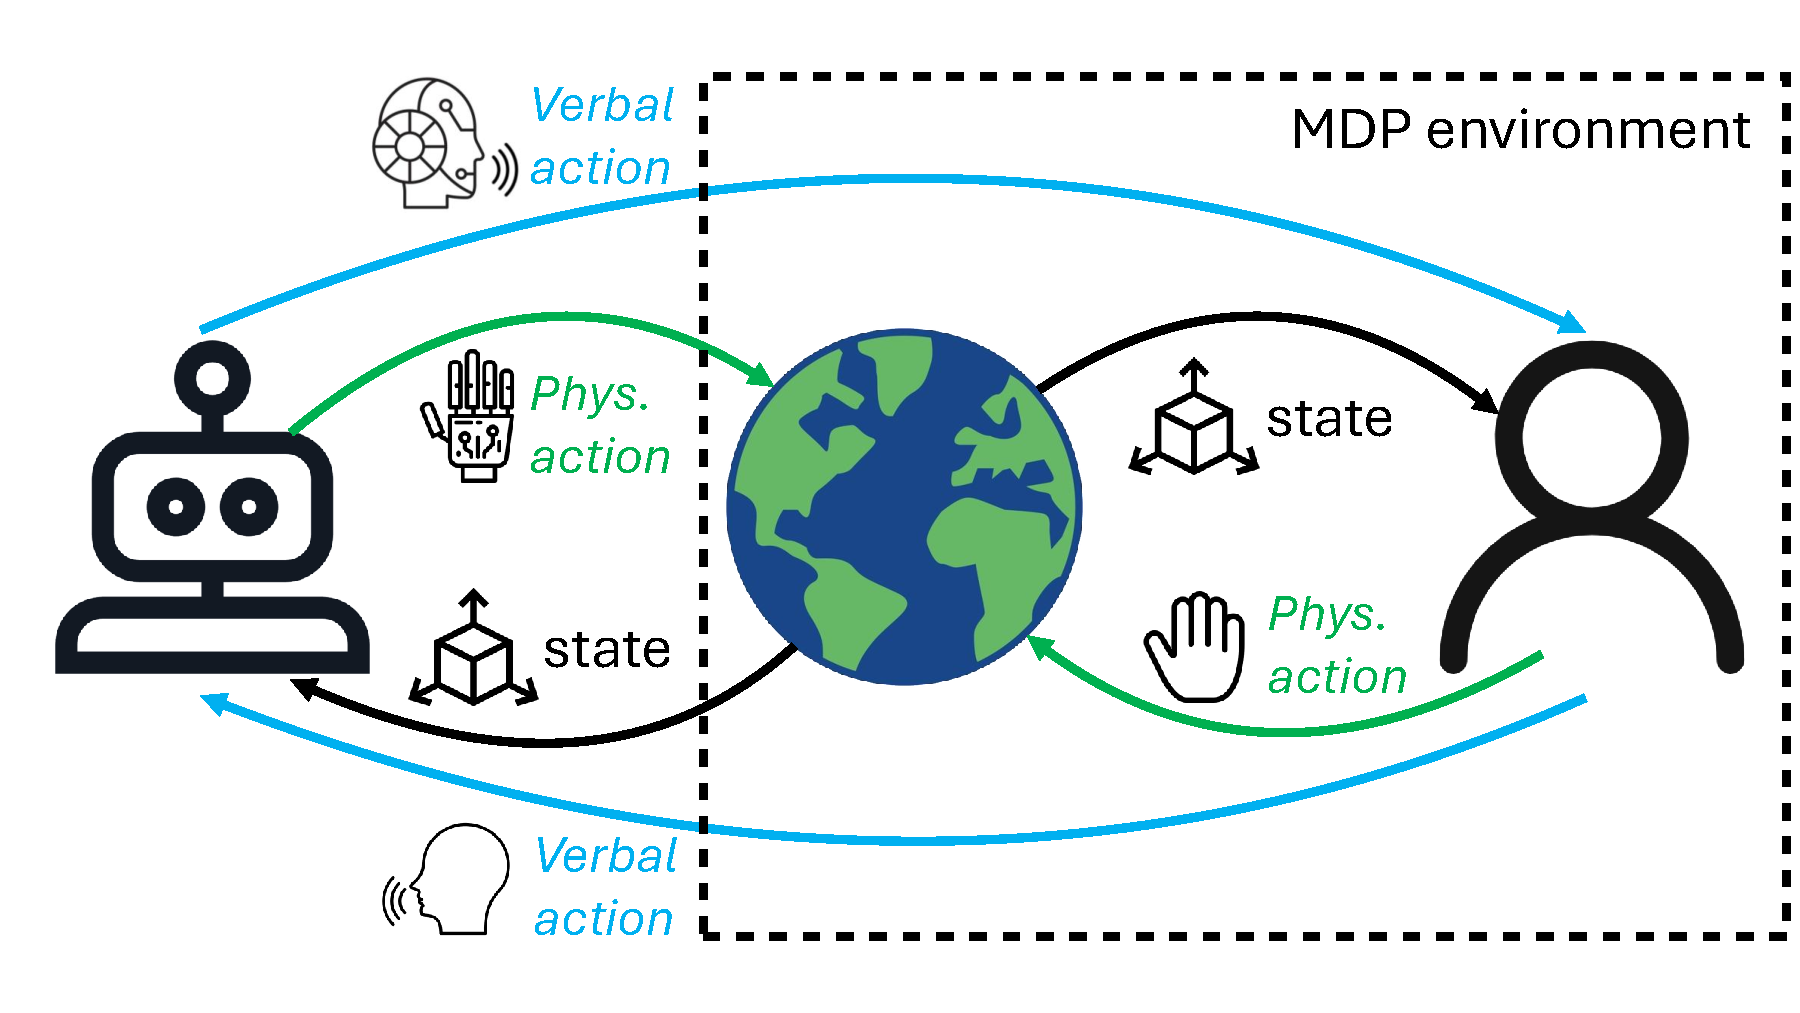
\includegraphics[width=\linewidth]{figs/fig2_v3.pdf}
%     \caption{Our MDP Formulation for Mixed-Initiative Collaboration}
%     \label{fig:mdp}
% \vspace{-10pt}
% \end{wrapfigure}
\vspace{-10pt}
\begin{figure}[ht!]
    \centering
    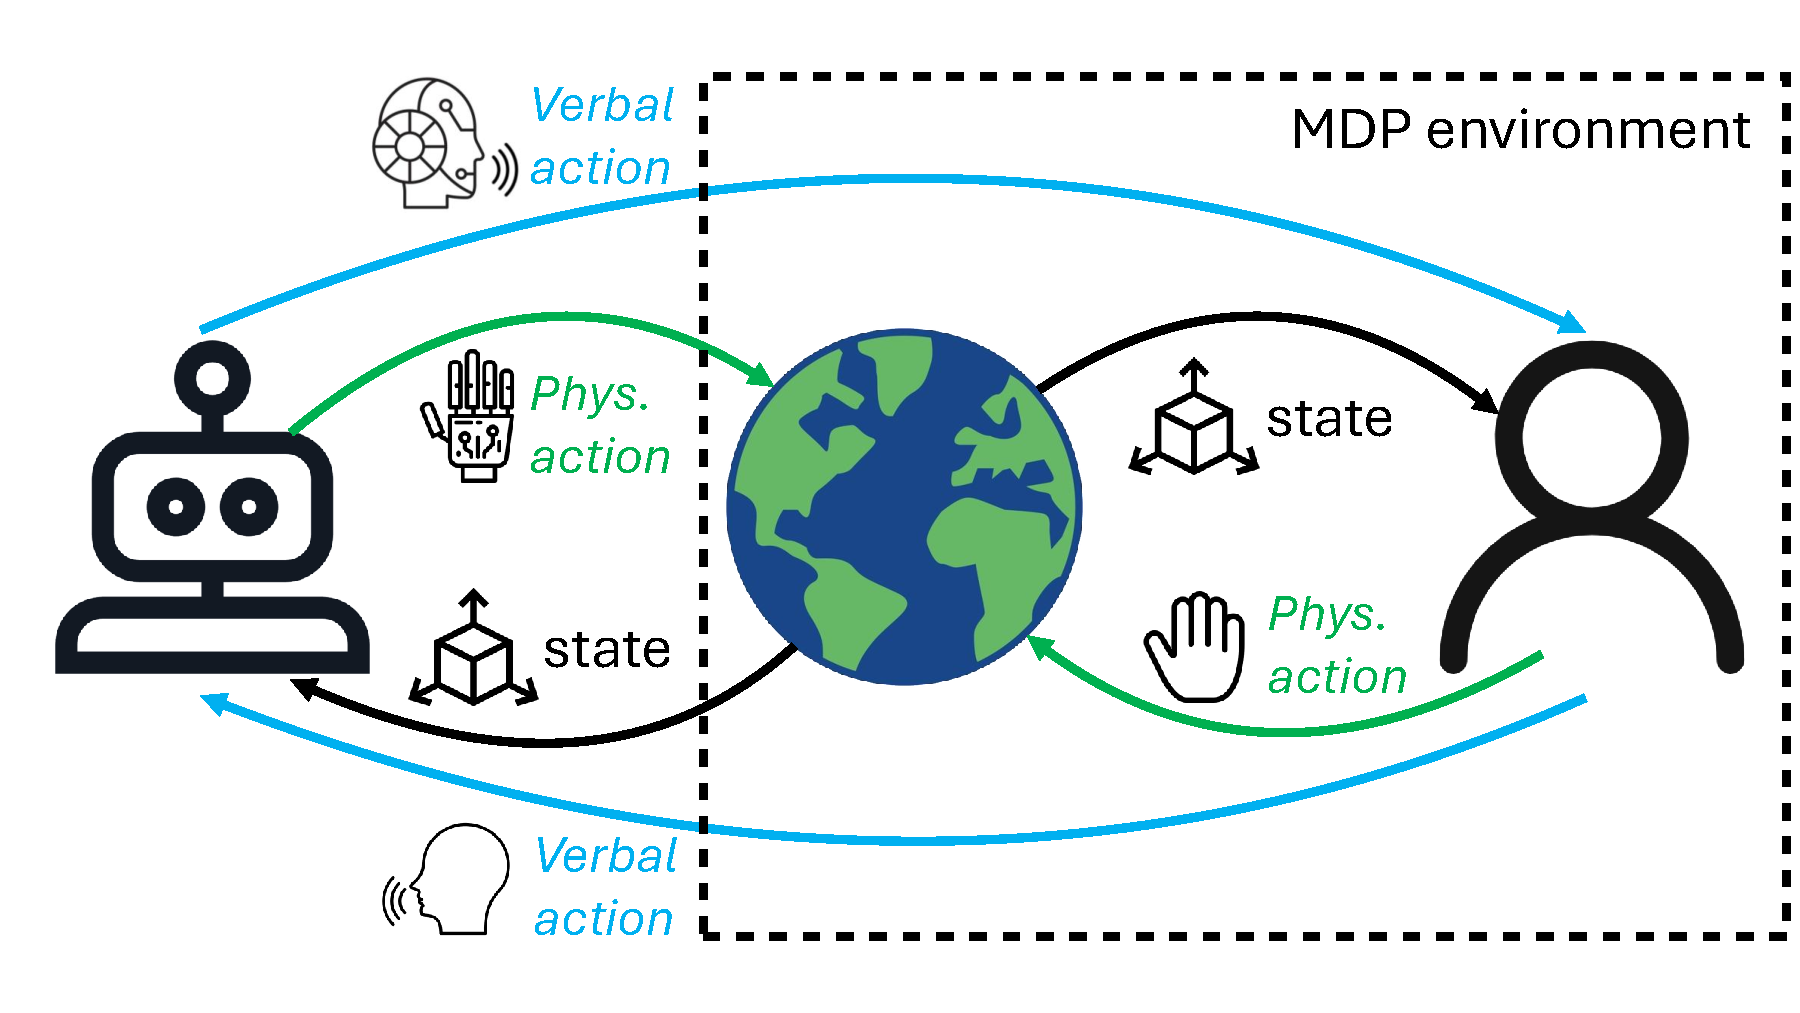
\includegraphics[width=\linewidth]{figs/fig2_v3.pdf}
    \caption{Proposed MDP for Mixed-Initiative Collaboration.}
    \label{fig:mdp}
\end{figure}

\textbf{MDP Formulation.} We study how human-robot collaborative manipulation can be facilitated through mixed-initiative dialog. We assume that both agents can observe the state of the world, $s\in\mathcal{S}$, and perform actions, % in a common action space of action primitives,
$a\in\mathcal{A} = \mathcal{A}_p \cup \mathcal{A}_v$, comprised of a physical action space, $\mathcal{A}_p$ (e.g., move objects, open them, etc.), that directly affect the physical state of the environment $s$, and a free-form, natural language verbal action space, $\mathcal{A}_v$, which is directly observed by the other agent but does not change the physical state. 
We model the problem as a Markov Decision Process (MDP) from the robot's point of view (see Fig.~\ref{fig:mdp}), where on each environment step, the robot performs some action, $a_R \in \mathcal{A}_{p, R} \cup \mathcal{A}_{v, R}$ and receives an observation $o = [I, a_{v, H}, s_\mathit{proprio}]$ consisting of an RGB-D image $I$, an optional verbal action from the human partner $a_{v, H}$, and the robot's proprioceptive state $s_\mathit{proprio}$. 
Within each environment step, the human may perform a series of actions, $a_H \in \mathcal{A}_{p, H} \cup \mathcal{A}_{v, H}$, in its own physical and verbal action space after perceiving the world state and robot's previous dialog, $a_{v, R}$.

\textbf{Physical and Verbal Action Spaces.} The physical and verbal action spaces, $\mathcal{A}_p$ and $\mathcal{A}_v$, are shared between both agents. Each element of these action spaces is a parameterized action primitive represented by the pair, $a_{p/v}=(\omega_{p/v},\theta_{p/v})$. $\omega_p$ is the type of the physical action primitive (\texttt{open}, \texttt{pick-and-place}, etc.) and $\theta_p$ are the corresponding parameters (e.g., what object to open or pick and where to place it). 
We assume that humans are fully competent in executing all steps of a collaborative household manipulation task but may be unwilling or unavailable to perform some or all required actions.
Their behavior can range from indifferent (never acting) to overly proactive (completing the entire task without robot involvement).

In contrast, robots often have limited manipulation capabilities and may be unable to execute more complex actions, in which case it uses verbal actions to communicate with the human.
$\omega_v$ is the type of the verbal action primitive (\texttt{ask\_human\_for\_help}, \texttt{respond\_to\_human}, etc.), and $\theta_v$ are the corresponding parameters defining the context of the verbal primitive (e.g., what step the robot needs help on).
While the types of verbal actions are limited, each generates freeform and open-vocabulary language. 
% Each verbal action can encompass multiple dialog intents, including both initiative and response.
\methodname{} first selects an abstract verbal action from this space, then translates it into a natural language utterance to negotiate with the human—conveying its requests and the assistance it requires for successful collaboration. This involves reasoning over asymmetric human and robot physical capabilities to devise collaboration strategies that maximize task success while minimizing human effort.

% generating the correct physical actions and translating them into low-level robot commands to perform its assigned subtasks.
% \roberto{check}We assume the robot's capabilities are a subset of the human's ($\mathcal{A}_{p, R} \subseteq \mathcal{A}_{p, H}$). We assume that the human is perfectly competent at performing all steps in the collaborative household manipulation task but may be unwilling or unavailable to perform any or all of them, ranging from indifferent (never performing any actions) to overly proactive (completing the entire plan without robot assistance). 
% Unlike the human, the robot is unable to perform the entire plan as there exists some $\omega_t(\theta_t)$ step it has 0\% success rate on, so the robot must work with the human to accomplish the whole task.

% \textbf{Verbal Action Space.} The verbal action space, $\mathcal{A}_v$, is also shared between both agents. 
% Similar to the physical actions, each element of the verbal action space is a parameterized action primitive represented by the pair, $a_v=(\omega_v,\theta_v)$, where $\omega_v$ is the type of the verbal action primitive (\texttt{ask\_human\_for\_help}, \texttt{respond\_to\_human}, etc.) and $\theta_v$ are the corresponding parameters that define the necessary context of the verbal primitive (e.g., what step the robot needs help on, or can/cannot perform).
% Depending on who initiates a sequence of verbal actions consider two main types of dialog initiative that both agents may engage in: (1) \textbf{Task allocation}, such as ``Could you please open the package?'' or ``I will bring the plate'', and (2) \textbf{Split proposal} to divide the next steps between the two agents, such as ``Can you bring me a pair of scissors so that I can use it to open the package?'' In response to these dialog initiatives, both agents may accept, refuse, counter-offer, or stay silent. 
% While the types of verbal actions are limited, the generated language based on them is freeform and open-vocabulary. Each verbal action can encompass multiple dialog intents, including both initiative and response.
% \methodname{} first selects an abstract verbal action from this space, then translates it into a natural language utterance to negotiate with the human—conveying its requests and the assistance it requires for successful collaboration.

\textbf{Collaborative Task Definition and Problem Statement.} 
We assume the collaborative task is defined by a task plan of length $T$, known to both agents and represented as a sequence of unassigned \textbf{physical} action primitives, $[a_{p,0}, ..., a_{p, T-1}]$, such as [(\texttt{pick-and-place}(\texttt{box}, \texttt{table}), \ldots, \texttt{close}(\texttt{box})], obtained from the task instructions or off-the-shelf task planner. 
% In the plan, $\omega_t$ are skill primitives that both agents could execute (e.g., pick or place an object) corresponding to actions of the physical action space, $\mathcal{A}_p$, and $\theta_t$ are the skill parameters that fully define each skill (e.g., the object to pick and where to place). 
% Each step of the plan is a skill-parameter pair, $\omega_t(\theta_t) \in \mathcal{A}_{p, R} \cup \mathcal{A}_{p, H}$.
To complete the manipulation task while minimizing human effort, the system must allocate steps of the plan between the two agents—negotiating with the human through robot-initiated dialog to suggest assignments, adapting to human preferences through human-initiated dialog, and ultimately executing its assigned physical actions.
At each step $t$, the system must compute the best allocation of the remaining steps of the plan, $G = [g_t, ..., g_{T-1}]$, where $\forall t, g_t \in \{H, R\}$. 
% so that all missing steps of the plan are assigned to the robot or the human, $[a_{H\backslash R,p,t}, ..., a_{H\backslash R,p,K-1}]$. 
% We assume that all plan steps are independent and self-contained, so that if one agent performs $\omega_t(\theta_t)$, either agent can perform the next step $\omega_{t+1}(\theta_{t+1})$. 
The optimal allocation $G^*$ maximizes the expected task success probability while minimizing total human effort.
These objectives are inherently competing: a policy focused solely on maximizing success might allocate all steps to the human (assumed to be perfectly competent); conversely, minimizing human effort alone would assign all steps to the robot, even when it may be incapable of completing certain steps.
The optimization also incorporates constraints conveyed through the mixed-initiative dialog history, such as task allocation requests or proposed task splits. %, and whether the other agent accepted, rejected, or counter-offered.
The resulting allocation $G^*$ determines whether the robot executes the current step ($R$) or negotiates with the human for assistance ($H$).

% \subsection{Optimization Formulation}
% \textbf{Collaborative Task Definition and Problem Statement.} 
% We assume the collaborative task is defined by a task plan of length-$T$ known by both agents and represented as a sequence of parameterized skills, $[\omega_0(\theta_0), ..., \omega_{T-1}(\theta_{T-1})]$. Such a plan can be generated by a task planner without knowledge of the collaborative setting~\cite{}. In the plan, $\omega_t$ are skill primitives that both agents could execute (e.g., pick or place an object) corresponding to actions of the physical action space, $\mathcal{A}_p$, and $\theta_t$ are the skill parameters that fully define each skill (e.g., the object to pick and where to place). 
% % Each step of the plan is a skill-parameter pair, $\omega_t(\theta_t) \in \mathcal{A}_{p, R} \cup \mathcal{A}_{p, H}$.
% The goal of our robotic system is to optimally divide up the steps of the plan between the two agents, negotiating with a human the parts they should perform (robot-initiated dialog) as well as adapting to human preferences (human-initiated dialog). The robot's objective at each step is to find the best allocation of the remaining steps of the plan $G = [g_t, ..., g_{T-1}]$, where $\forall t, g_t \in \{H, R\}$. We assume that all plan steps are independent and self-contained, so that if one agent performs $\omega_t(\theta_t)$, either agent can perform the next step $\omega_{t+1}(\theta_{t+1})$. The optimal allocation $G^*$ maximizes the expected task success probability while minimizing total human effort.
% These objectives are inherently competing: a policy focused solely on maximizing success might allocate all steps to the human (assumed to be perfectly competent), thereby eliminating the robot’s assistive role; conversely, minimizing human effort alone would assign all steps to the robot, even when it may be incapable of completing certain tasks.
% The optimization must also incorporate constraints conveyed through the mixed-initiative dialog history, such as task allocation requests, proposed task splits, and whether the other agent accepted, rejected, or counter-offered.
% The resulting $G^*$ determines whether the robot executes the current step or instead asks the human for assistance.


% We work in a human-robot collaborative scenario, where the human $H$ issues a natural language task instruction to the robot $R$.
% For a given language-specified long horizon task, we assume access to a length-$T$ plan $[\omega_0(\theta_0), ..., \omega_{T-1}(\theta_{T-1})]$ of skills $\omega_t \in \Omega$ (such as pick-and-place, opening, pouring), and a tuple of parameters $\theta_t$ (such as the object to pick and where to place, the object to open, etc).
% The robot is capable of executing a subset of the skills in the plan with various success rates. We assume a non-adversarial human collaborator that ranges from indifferent (never talks or helps the robot), to proactively---and potentially overly---helpful and verbose.

% At every environment step, the robot can either engage in a verbal action (speaking freeform language to $H$), or perform the next physical skill-parameter pair $\omega_t(\theta_t)$ in the plan. The human can also perform either verbal or physical actions in the environment, with the only difference that it can perform multiple physical actions or dialog actions in a single environment step. The human is assumed to perform each step of the plan competently if it has agreed verbally to perform a step.

% There are four possible dialog types that both agents can engage in and initiate at any environment step: (1) \textbf{Task allocation}, such as ``Could you please open the package?'' or ``I will bring the plate.'' (2) \textbf{Acceptance or refusal}, such as ``No, I'm too busy to do that,'' or ``I'll be super happy to help!'' (3) \textbf{Split proposal} to split up the steps between the two agents, such as ``How about you bring me a pair of scissors so that I can use it to open the package?'' and (4) \textbf{Silence}. Either agent can refuse to respond to the other's dialog at any given time.